\documentclass[11pt]{article}
\usepackage{graphicx}
\usepackage{amsmath}
\usepackage[utf8]{inputenc}
\usepackage{setspace}
\usepackage{caption}
\usepackage{subcaption}
\usepackage{wrapfig}
\usepackage{caption}
\captionsetup[figure]{font=footnotesize}
\usepackage{lineno}
\usepackage{harvard}
\usepackage{parskip}
\usepackage[a4paper,width=150mm,top=20mm,bottom=20mm,bindingoffset=6mm]{geometry}

\doublespacing

\begin{document}

\begin{titlepage}
    \begin{center}
    \vspace*{1cm}

    \Huge
    \textbf{\underline{Modelling the effects of Gene Flow and Selection on the Canalisation}}\\
    \textbf{\underline{of an established Genetic Network}}\\

    \vspace*{2.0cm}

    \large
    \textbf{Author: Matthew Campos}\\
    \textbf{Submitted August 2020}

    \vspace*{0.8cm}

    \normalsize
    A thesis submitted in partial fulfilment of the requirements for the degree of Master of Science/Research at Imperial College London\\
    Formatted in the journal style of Evolution \& Development\\
    Submitted for the MSc in Computational Methods in Ecology and Evolution\\

    \vspace*{0.8cm}

    \end{center}
\end{titlepage}


\newpage

\linenumbers

\section{Six Keywords}
Gene Flow, Gene Regulatory Network, Robustness, Local adaptation, Epistasis, Alleles

\section{Introduction}
Societal progress has caused anthropogenic changes, many of which will have harmful long-term effects to species. In addition, geological changes will lead to shifts in the distribution of land and alteration of habitat states. One effect of this change can be migration. Whether it is forced migration or new route opportunities, the distribution and movement of species will change over time. These migrations can cause the introduction of novel genes into local habitats, implicating future evolutionary effects in these local habitats. Evolution of both the local species and migratory species. The presence of these novel suboptimal genes, along with the interaction of species in the environment will lead to evolutionary change. After many generations, this change will be seen in a phenotypic level as well as genotypic.

Gene interaction within and across loci can result in robustness, from the effects of epistasis, additivity and dominance, all of which are connected \cite{omholt2000gene}. The concern is on how a network responds to the effect of gene flow, seeing the evolving genetic interactions. Previous research looked at its effects, with selection and mutation generating local adaptation at the phenotypic level. This shows how maintenance of alleles and linkage is important in adaptation \cite{yeaman2011genetic}. Furthermore, random perturbations and genetic modifiers limit the bounds for which selection for canalization can act on, leading to evolution of robustness. When species are under migration selection balance, selection for robustness increases with the migration rates \cite{proulx2005opportunity}. The purpose of the research will be looking at the change in genetic architecture dynamics and structure with the interactions of the systems that maintains this robustness. Furthermore, as the network evolves, it has been shown that there exists a threshold which is actively regulating these homeostatic genes \cite{gjuvsland2007threshold}.  As selection of robustness occurs within the local population, it can give insight into the change in architecture and statistically significant interaction \cite{gjuvsland2007statistical}. Using computer models, we can simulate the effects over many generations and see how the output of the network changes, looking at allelic interaction and possibility of epistasis and dominance.

\section{Proposed Methods}
Using software packages including RStudio, SLiMgui, I will write an algorithm to run simulations to see the effects of gene flow on a population, looking at the changes at the genetic level. Using a well understood gene network as a model system to represent one population, another model population will be introduced to run simulations of migrations and see the evolution of the model network. This model system can either be of small scale, containing one or two genes, intermediate scale of around 10 genes or a whole genome. The populations are not representative of any specific species but rather just to see the effects over many simulated generations.  The well understood network will be the model system in which gene flow is introduced. The focus is solely on the effects of migration and genetic adaptions, thus environmental influence will not be considered in these simulations. However, stochasticity such as mutation will included in the model.

\section{Anticipated outputs and outcomes}
With the introduction of gene flow in the gene network, the anticipated output would be an evolved network with different dynamics and interactions from the start. The expectation is that with gene flow, genetic interaction will cause a change in genetic polymorphisms, and allelic and loci interaction. Selection for canalization will lead to a more robust network with the possibility of different alleles, allelic frequency and gene interactions. With the effects of epistasis, it is possible that the locus selecting for robustness is influenced by another locus in the network, and the latter locus is the one evolving.

\section{Project feasibility supported by a timeline of tasks}
\begin{figure}[h!]
\centering
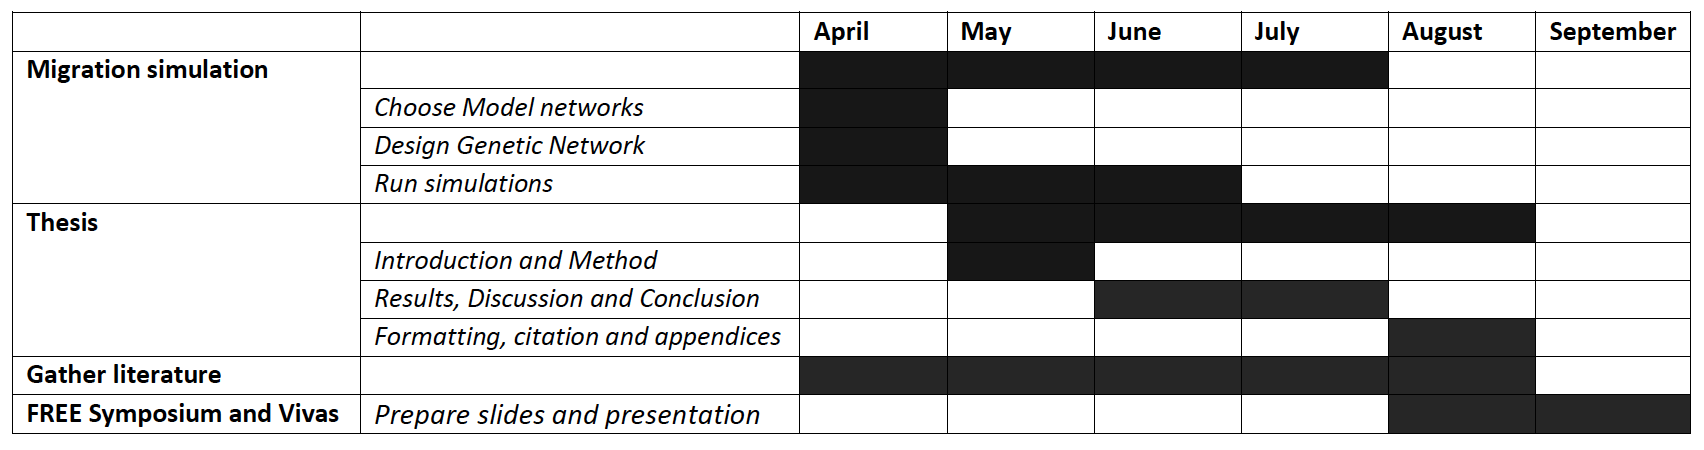
\includegraphics[scale=0.35]{Gantt_chart.jpg}
\caption{Gaant Chart showing projected schedule}
\label{tab:Gantt Chart}
\end{figure}

\section{Itemized Budget}
\$500 for the travel

\bibliographystyle{agsm}
\bibliography{references}

\newpage

\textbf{I have seen and approved the proposal and the budget}\\
Thomas Bell   16/3/2020\\
-----------------------------------------------------------------------\\
Name and date

\end{document}
